\chapter{Background}

\label{Chapter2}

This section will present the main concepts that are relevant to the thesis project and the reason why it's useful.
It will first explain the main theory behind microservices and how it seeks to solve the main problems in legacy software architectures. Then it will
detail the new issues that arise from microservices. Finally, it will paint a picture of today's landscape of distributed software and 
tie it all together to explain the value of the research in this project.

\section{The monolith}
In general when talking about both microservices and distributed computing in general, the concept of a \textbf{Monolith} often gets brought up. 
The monolith is this concept of a large, self-contained application where all the code and functionality is tightly bundled together, and is very hard to separate into individual parts.
The definition has changed over time: According to the ITS back in 2001 \cite{ITS}, a monolith was "An application in which the user interface, business rules, and data access code is combined into a single executable program and deployed on one platform."
However, most modern interpretations online refer back to a book from 2003 called \textit{The art of Unix programming}. Usually referred to as "monster monoliths", it marks the beginning of the trend of using the term monolith as a bogeyman of unmaintainable, poorly planned code. 
This trend has been continued in modern days with software "gurus" and the like when needing something to compare to our lord and savior microservices \cite*{Gouigoux2017}.
It is therefore important to remember that:
\begin{enumerate}
    \item The monolith is not a defined software architecture design paradigm. Rather, it is the default type of application that appears when not taking great effort and intentionality to split the code up in many distinct parts.
    \item The monolith is not some damnable evil to be conquered: On software projects of a less-than-huge scale, it is very often quite optimal. It doesn't have to deal with inter-component communication. Keeping everything contained in one code base makes it easy to run and test on local machines, keeps all the code in one place for easy access, and so on. 
    \item The monolith mostly just exists as a concept when talking about microservices or other ways to break it up. Its purpose is mainly to demonstrate the benefits of code splitting in large software.
\end{enumerate}

With that out of the way, let's discuss the problems with monolithic software that microservices seek to amend.\\
The core issue that with monolithic software is \textbf{entanglement.}
In this context, it means how complex monolithic software will have too many interconnected, interdependent parts to manage effectively.
This interdependence will mean that something that is a problem for one small part of the whole, will be a problem for the entire tech stack. 

\subsection{Scalability} 
Scalability refers to the ability to increase the workload capacity of the software \cite*{Scalability}. 
If the amount of users, data, geographical reach or computation complexity increases, it becomes necessary to increase hardware capabilities. 
Scaling up monolithic software can be a time-consuming and costly affair, as it usually doesn't allow for only increasing the capacity of the parts of the software that are facing increased load.  \\
An example: 
\begin{quote} 
 On the 24th of December 2004, Delta Air Lines' crew scheduling system crashed because of an integer overflow bug resulting from record system load. 
 It took 24 hours of frantic work to implement a workaround that duplicated a database \cite*{USAToday}. 
It used an old flight scheduling system called TRACK from 1986 to organize scheduling. 
Their database that handled pilots and flight attendants ran into a hard limit at 32000 entries.
The hotfix for this problem was to spin up another server, and let one database only handle pilots and another only handle flight attendants. 
The crash caused widespread disruptions. According to the Department of Transportation of the US, approximately 269,000 passengers were affected by delays and cancellations \cite*{DOT}. 
\end{quote}
Issues from heavy loads like this are always a risk. But entangled monolith systems are not easy to extend. 
In a microservices oriented system, implementing this extension fix would likely be on the scale of modifying a few lines of code and spinning up another instance of the database. 
I highlight this example because the fix for this huge problem ended up being a basic principle of microservices: Generating more instances of only the overloaded components. 
\\
When an application has reached load capacity, one realistically has two options \cite*{Scalability}:
\begin{enumerate}
    \item Improve the efficiency of the software, so it can serve higher loads with the same hardware
    \item Upgrade the hardware
\end{enumerate}
Naturally, the software improvement solution will only get you so far. It has the added issue of (in this example) being a monolithic application, so big changes to the software is a time consuming and costly project.\\
When upgrading the hardware capacity of monolithic applications, it often becomes a project of its own. One with expenses. 
Because of this, and the fact that monolithic application will have to be replicated in its entirety on the new server by default, a scaling project will try to calculate the future growth of the user base and invest in a solution that will be able to handle user load for the foreseeable future.
This is a point of potential failure, as being wrong about future growth could turn out to be quite costly.
\begin{figure}[ht] 
\centering 
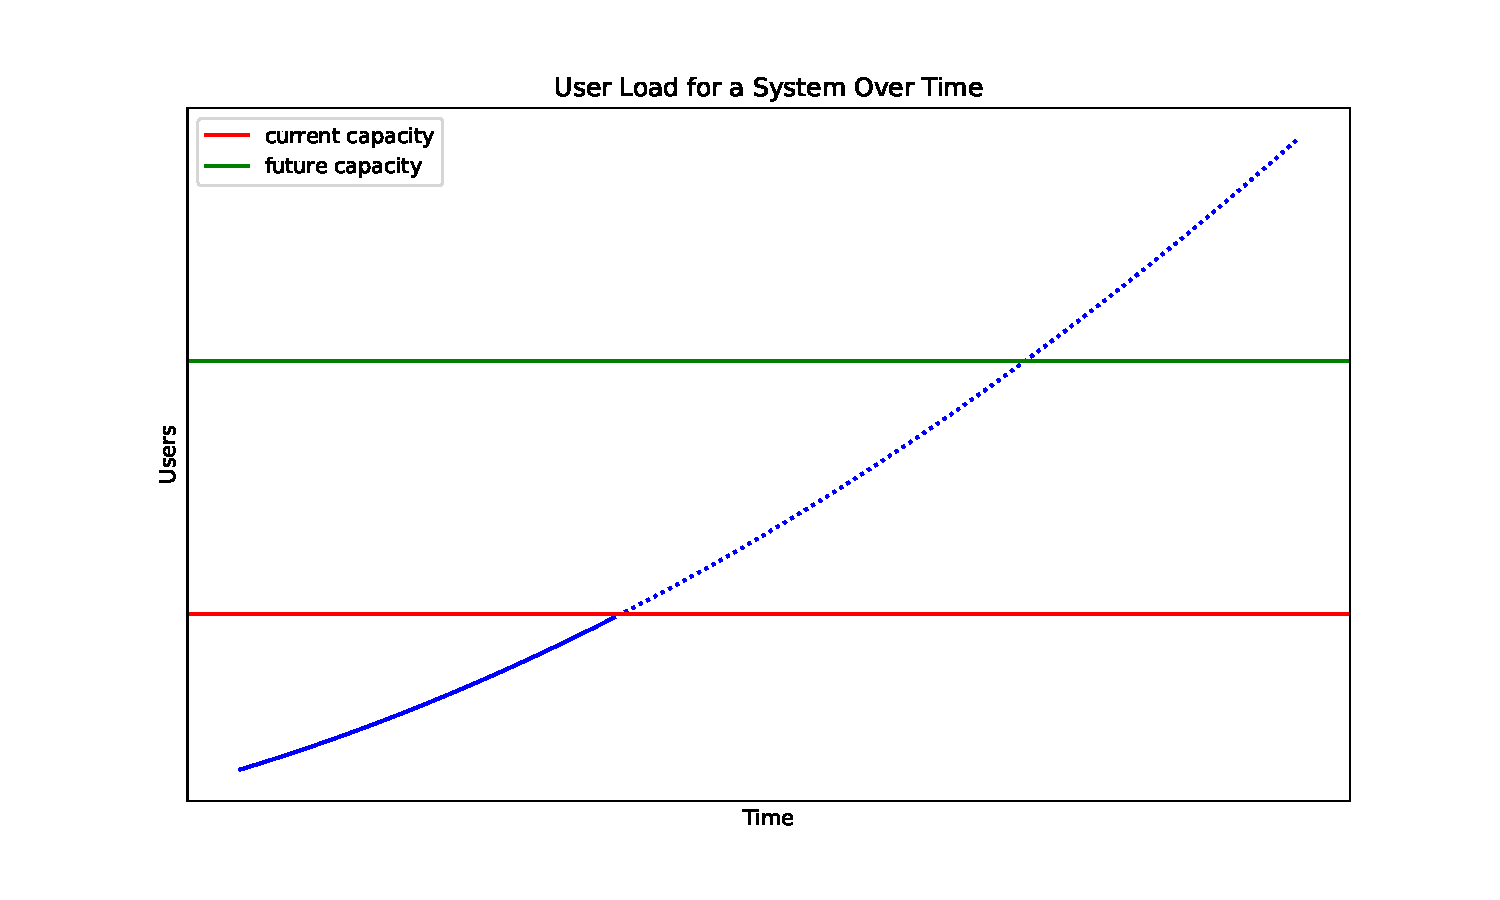
\includegraphics[width=0.8\columnwidth]{Figures/Graphs/capacity_scaling.pdf}
\caption{Scaling a monolith requires making assumptions about future growth}
\label{Monolith scaling}
\end{figure}

\subsection{Comprehension}
Comprehension of large software is impossible. 
There is a human limit to how much one can keep in one's mind. 
In large software, the amount of functions and interactions can balloon into the tens or hundreds of thousands. 
Fully comprehending such a system is impossible for human brains, and it becomes necessary to abstract it down to a manageable mental model. 
Without good comprehension of the system, it is very difficult to make good changes, adjustments or additions.
A highly entangled monolith can very difficult to abstract, without clear boundaries for which parts do what.

\subsection{Modern software development}
Modern software development is characterized by autonomous teams working separately and collaborating through continuous integration. 
This means: build often, test often, merge often. 
According to Agile practices, one should write tests first, then write code that passes the tests. 
But writing tests for highly entangled monolithic software is challenging, as even small changes can have consequences far down the chain. 
Building often will also become costly: Monolithic software will typically need to be rebuilt from scratch each time. 
A costly affair, and entirely unfeasible if the goal is to build several times a day. 

\subsection{Resilience}
Resilience has several definitions in the context of software. \cite*{Curtis}. 
In the context of this thesis, we can define it as "the ability to keep running correctly in spite of failures". Often called fault tolerance.
The entanglement of the monolith once again becomes a problem here. 
A single function running into an unexpected situation and throwing an error will, by default in most technologies, abort the execution of the program entirely.
It can be circumvented by try/catch statements and other error handling methods, but an entangled system is extremely difficult to make fault tolerant.

\subsection{Technical debt} 
Technical debt is a somewhat loosely defined term. It is defined by Steve McConnell as \textit{A
design or construction approach that's expedient in the short term, but
that creates a technical context in which the same work will cost more
to do later than it would cost to do now (including increased cost over
time) \cite*{McConnell2013}.”}
As a monolithic application grows, making any change becomes a larger project.
The more entangled everything is, the more changes will have to be made to accommodate updated dependencies or changes in behavior. 
These changes to accommodate the change can also cause other things to be changed.
This is often called the "ripple effect" or "cascading changes". 
This can lead to mounting technical debt: As updating components is such a project, it is delayed, or jury rigged to work in the short term.
But each delay or subpar implementation leads to an increase in how big of a project it would be to properly update dependencies.
Technical debt will also make regular maintenance more difficult and time consuming over time. 
Technical debt is not a problem that is unique to monoliths. 
But it is hard to pay off that debt through refactoring and maintenance in an entangled system that handles change poorly.

\section{Containers}
Containers are a technology that packages a unit of software and all its required dependencies.
They make use of the Linux kernel's namespaces feature.
Namespaces partition system resources in a way that processes only "see" the resources in their namespace, instead of the total system resources. 
This provides a level of abstraction and security, as processes can only access their own namespace.
By utilizing namespaces, containers can provide isolated workspaces for processes, essentially allowing applications to run in their own "virtual" system, oblivious to other processes running on the same host.
This makes containers completely dependency and OS agnostic,
since each container comes with the OS and packages they need to run their process.
Containers are similar to virtual machines, but much faster and more lightweight.
VMs virtualize the hardware and entire OS, like RAM and the kernel, and then run their OS on the virtualized hardware. 
Containers simply virtualize the OS, running it on their assigned namespace on the host's kernel.
This takes far fewer system resources at a slight cost to isolation.
This makes them viable as a way to organize code segments.
Containers talk to each other using regular network calls. 
Because of this, an application can freely be split up between several machines.

\begin{figure}[ht] 
\centering 
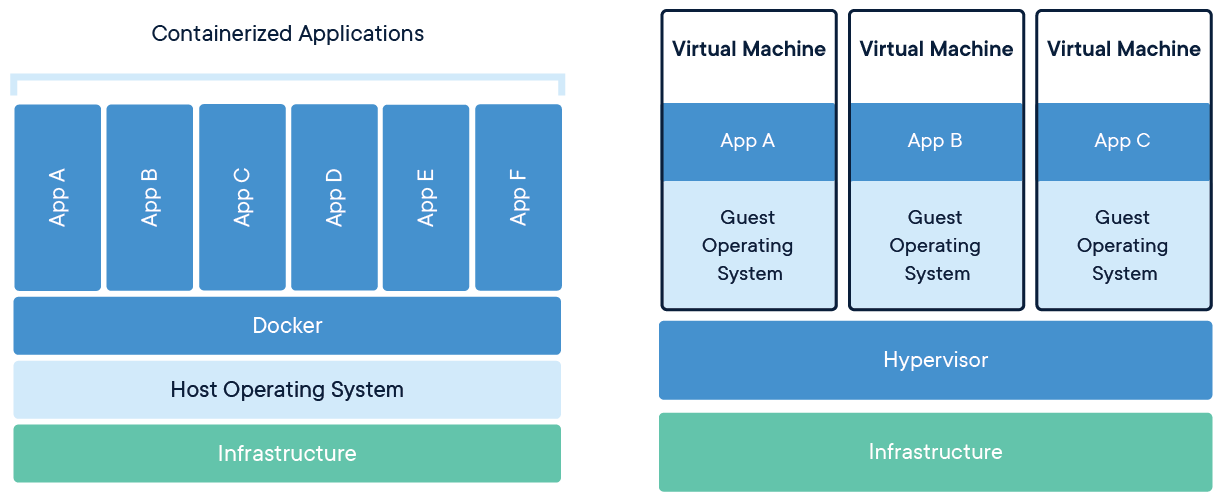
\includegraphics[width=\columnwidth]{Figures/containers_vs_VMs.png}
\caption{Containers vs VMs. Image credit: Docker inc}
\label{Containers}
\end{figure}


\section{The microservice}
The core idea of microservices is modularization, which has been a concept in software engineering since its inception. 
Microservices are a modern spin on the concept with cloud and DevOps in mind. 
The defining feature of the microservice is the container. 
By splitting the code of a piece of software into several autonomous containers that talk to each other using web requests, 
one can counter a majority of the problems with large software projects. \\
Let's examine how microservices tackle the main problems with monolithic software.

\subsection{Scalability}
Microservices are designed to be very easy to scale. 
Because the containers in a microservice system talk to each other using network calls anyway, a microservice system does not particularly care \textit{where} the containers are located.
This means you can gracefully distribute the software across servers and spin up only however many instances of each microservice you need.
This works well with modern server renting solutions, that let you pay for only what you need. 
In this way, the aforementioned scaling project for monoliths that try to calculate future growth becomes unnecessary. 
One can simply scale out only what one needs, when one needs.

\begin{figure}[ht] 
    \centering 
    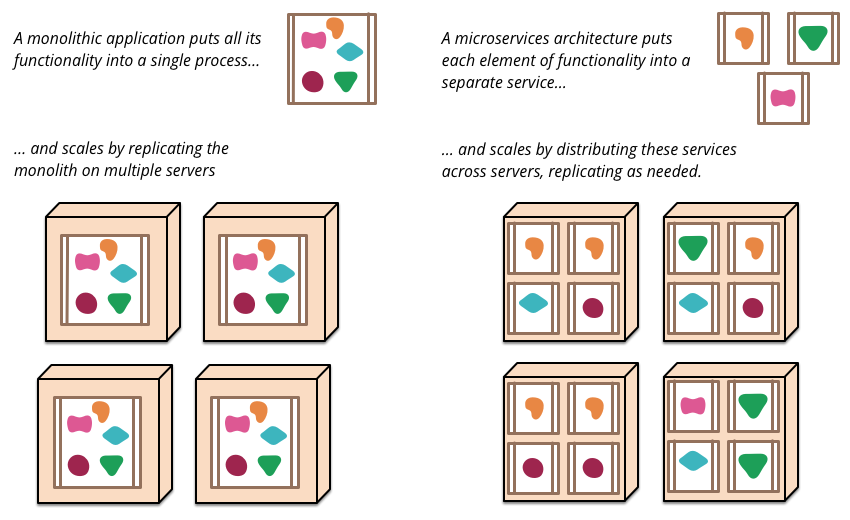
\includegraphics[width=\columnwidth]{Figures/scaling.png}
    \caption{Illustrating how monoliths and microservices handle scaling. Credit: Martin Fowler \cite*{Fowler2014}}
    \label{Scaling-comparison}
\end{figure}

\subsection{Comprehension}
Microservices promise to make complex software easier to work with. 
It does not typically do this by reducing complexity, but by providing real, traceable boundaries between units of software, and by use of interfaces.
By software boundaries, I mean that developers have an objective rule to follow for breaking code up into pieces that can be mapped out and abstracted.
Without microservices one can still map out a program, but the boundary lines between units can often be hard to nail down in a satisfying manner.
Functions are a natural "unit" to break a program up into, but functions vary a lot in size, scope, and utility.
Mapping out a program or its states, for example in UML, requires reasoning about a level of abstraction to use in the current map context. 
This decided level of abstraction will likely need to represent some functions by themselves, while grouping others together. 
While this is not necessarily a bad thing, it makes the process of mapping out a program require skilled, subjective reasoning. 
Microservices, on the other hand, provide an objective boundary that makes sense in the context of mapping out a program to comprehend it.
Thus, as long as the microservice architecture itself is well thought out (which is not guaranteed at all), no skill is necessary to create a logical abstraction of the system that is guaranteed to be useful for comprehension.\\

Interfaces are the intended inputs and outputs of each microservice. 
They help comprehension by letting developers think of the rest of the program as a black box, and only focus on comprehending the parts of the program that interact with the microservice they are currently working on.
They don't have to know what the entirety of the system does to make good changes (in theory).

\subsection{Modern software development}
The modern day is a time of DevOps and agile development.
The core principles of DevOps is up for some debate \cite*{Devops-definition}, but can be roughly summarized to be a set of guiding principles to facilitate communication and collaboration between developers and operators (hence the name DevOps). 
It places emphasis on continuous integration, delivery, and deployment (CI/CD). 
Microservices are often regarded as a core component of DevOps \cite*{Devops-amazon}.
The independence of microservices aligns well with DevOps principles. 
Each service can be developed, tested, deployed, and monitored independently, allowing for more frequent updates and releases. 
This plays into the CI/CD model central to DevOps: updates are continually integrated into the software, tested, and then deployed. 
By breaking down the application into smaller services, teams can manage and maintain their CI/CD pipelines more effectively, each focusing on their own service.\\
\\
Microservices also fit well within Agile methodologies. 
Agile focuses on iterative development, where software is developed in small pieces, with stakeholder feedback incorporated along the way. 
Microservices support this iterative approach by allowing teams to work on different services simultaneously.
\subsection{Resilience}
The ability to handle faults, crashes and unexpected occurrences is crucial to modern software platforms that provide necessary services to large parts of the population. 
Modern microservice technologies and services, like Kubernetes, OpenShift, Rancher, Google Kubernetes Engine (GKE), Azure Kubernetes Service (AKS), and many more, provide automatic load balancing and self healing. 
This means that they will detect faults and spin up new instances of the microservices to take over the workload of the failing service. 
This makes microservice applications much more robust than monoliths, which are constantly at great danger of letting a single fault bring the whole service down.

\subsection{Technical debt}
The way microservices help deal with technical debt is by making it easier in general for developers to make changes and adjustments to the system.
That is to say, technical debt will accumulate in microservice architecture just like it does in monoliths. 
It is just that the more robust and changeable microservice system is easier to refactor individual parts of the system.
This is achieved through the total separation of components that talk to each other through \textbf{interfaces}. 
The interface in this context just means the expected inputs and outputs of each microservice.
Each individual microservice is "blind" to what goes on in the others, and treat them as black boxes.
All they care about is the interface: If what goes into a service and what comes out of it has the same properties as before, a microservice system will not notice a change even if the entire technology stack of the microservice is replaced.
This makes updating to new technology a much simpler process: A developer just has to make sure it can receive and send the same data as before, and not worry any further about ripple effects.

\section{The problems with microservices}
Microservices solve many problems with legacy software, but it also introduces issues of its own. 
The problems that microservices create have largely to do with complexity.
The reality is that microservices aren't less complex than monoliths, they just exchange one type of complexity for another. 
One that, it is argued, is easier to deal with. It leads to issues nonetheless.
This section will give a detailed overview of the problems that microservices introduces.

\subsection{Complexity}
Microservices do not reduce complexity: They simply exchange one type of complexity for another. 
The issues with complexity in microservices come from the architecture itself, and from the fact that it is so loosely coupled that it allows for any technology stack and programming language.\\
Microservice has to orchestrate and manage many, many nodes. 
The scaling method of creating more instances of microservices that are struggling to handle load is great for easy scaling, but it can easily become a nightmare to manage.
When multiple instances of the same service are to cooperate, care has to be taken to split the workload in a good manner.
Careless management can lead to race conditions, data getting lost, or tasks being done several times in a redundant fashion.\\
Larger systems will have hundreds or thousands of microservices that need to communicate with each other in a complex web that is difficult or impossible to comprehend.
Orchestrating and managing this complex web of web requests is a field still in development.

\subsection{Communication overhead}
The decoupled nature of microservices comes at a concrete cost in communication overhead.
If one compares two equally well made services of equal function and size, one running on a monolith and one on microservices, the monolith should have less latency and better performance.
The cost of communication is twofold: Complexity (as mentioned above), and resource usage.
There are ways to organize connection complexity, like event-driven architecture (EDA), service mesh solutions (Istio, Linkerd, Cosnul) or serverless architecture solutions like AWS Lambda, which abstract the network away from the developer entirely.
But all of these solutions need computing power and bandwidth to work, which means they come at a cost of performance. \\
There is also the issue of the various units of code communicating with each other through network requests.
This is, in many ways, the secret sauce that makes microservices so reliable and scalable. 
But function calls are faster and less resource intensive than network requests by an order of magnitude. 
Internal function calls just deals with local memory, and their speed is measured in nanoseconds.
Meanwhile, network requests are typically measured in milliseconds. 
The distributed nature of the microservices also mean that a service could be needing to communicate with another server on a different place on the planet.
This is also a significant factor for latency, and can be a bottleneck for service quality.


\subsection{Data consistency}
\begin{wrapfigure}{r}{0.5\textwidth}
\centering
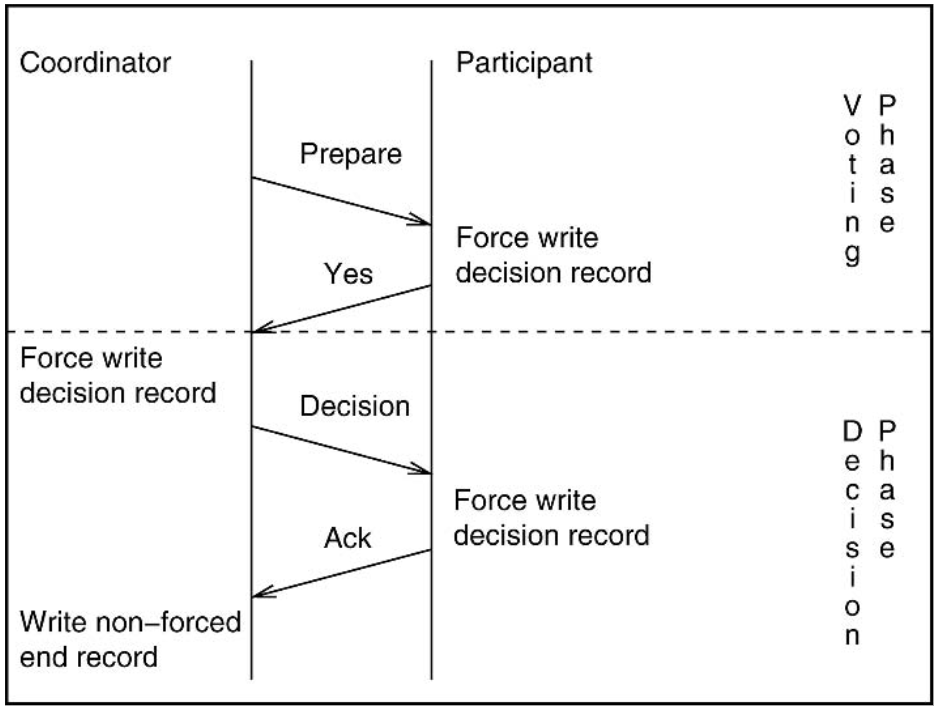
\includegraphics[width=0.48\textwidth]{Figures/two_phase_commit.png}
\caption{The two-phase commit protocol. Credit: \cite*{Samaras2009}}
\label{2PC}
\end{wrapfigure}
Data consistency (and the lack thereof) is another complexity trade-off in microservices architecture.
While implementations vary, it is common for microservices to each have their own little database for storing data relevant to their work.
This leads to resilience, but also means that changed values may take time to propagate to all relevant microservices, leading to microservices potentially disagreeing on the value of certain variables.
This can lead to inconsistent data, where an end user might get a different result depending on time of day or where they are pinging the service from.\\
Updating data can be a challenging affair. If, for example, there is a network of 100 microservices that need to be updated with new data, that is 100 potential points of failure.
If data consistency is important, changes would need to be rolled back if any of the 100 transactions fail. 
That would require noticing a fault occurred, then notifying all the services that changed successfully that they must roll back, introducing more potential points of failure.
The most common implementation of this is the \textit{two-phase commit protocol} (2PC). 
It works by assigning one node as the coordinator/master, who sends a query to commit message to all other nodes.
All nodes then vote, by performing some internal check to see if it could successfully commit the proposed change.
This is the first phase of 2PC, the voting phase.
If all nodes voted yes, then a commit message is sent from the coordinator/master to perform the change.
This is phase two of 2PC, the decision phase.
This process does a pretty good job at ensuring data consistency, but has many potential issues.
While the core algorithm itself is pretty simple, the actual implementation ends up being complex because it has to include protocols for many types of issues \cite*{Samaras2009}.    


\subsection{Testing and debugging}
Microservice architectures can become very complex. As stated earlier, it is an intentional complexity trade-off that should be more manageable in theory.
Their specific brand of complexity gives rise to a specific brand of headaches for testers and developers.
The complex network interactions between independent nodes create new potential points of failure that can be hard to track and debug.
